% !TeX spellcheck = cs_CZ

\documentclass[a4paper,11pt]{article}

\usepackage[a4paper, left=1.5cm, right=1.5cm, top=1.5cm, bottom=2cm]{geometry}

\usepackage[czech]{babel}
\usepackage[utf8]{inputenc}
\usepackage[T1]{fontenc}
\usepackage{amsmath}
\usepackage{amsfonts}
\usepackage{amssymb}
\usepackage{wasysym}
\usepackage{textcomp}

\usepackage{graphicx}
\usepackage{wrapfig}
\usepackage{enumitem}
\usepackage{fancyhdr}
\usepackage{index}
\usepackage{lmodern}

\usepackage{hyperref}
\hypersetup{colorlinks}
\urlstyle{same}

\usepackage{listings}

\usepackage{siunitx}
\usepackage{multirow}
\usepackage{longtable}
\usepackage{translator}

\usepackage{multicol}
\usepackage{booktabs}
\usepackage{caption}

\newcommand{\iu}{\mathrm{i}}
\newcommand{\konst}{\mathrm{konst.}}
\newcommand{\dif}{\mathrm{d}}
\newcommand{\eul}{\mathrm{e}}
\newcommand{\tens}[1]{\mathbf{\hat{#1}}}
\renewcommand{\vec}[1]{\mathbf{#1}}

\newcommand{\ket}[1]{|#1\rangle}
\newcommand{\bra}[1]{\langle#1|}
\newcommand{\mrm}[1]{\mathrm{#1}}

\newcommand{\init}{\mathrm{i}}
\newcommand{\fin}{\mathrm{f}}

\newenvironment{Figure}
{\par\medskip\noindent\minipage{\linewidth}}
{\endminipage\par\medskip}







\sisetup{output-decimal-marker = {,}, group-minimum-digits = 4, inter-unit-product =\cdot, exponent-product= \cdot, per-mode = reciprocal}
\sisetup{range-phrase=--}
\sisetup{separate-uncertainty=true,
	list-final-separator = { a~},
	list-pair-separator  = { a~},
	range-phrase         = { \ \mathrm{až}\ }
}






%\pagestyle{fancy} %						Hlavička
%\rhead{Martin Ošmera (208392)}
%\lhead{TQS -- Zápočtový úkol}
%\chead{\today}
%
%
%
%\author{Martin Ošmera (208392)}
%\title{Zápočtový úkol do kvantové mechaniky \\
%	\textbf{22. Vlnový balík dopadající na dvojitou potenciálovou bariéru s~maximem vyšším než je energie balíku }  }
%\date{\today}






\begin{document}
	
	%\maketitle
	%\thispagestyle{plain}
\begin{center}
	
	\today, Martin Ošmera (208392)
	\vspace{2mm}
	
	{\Large TPX -- Plánování a vyhodnocování experimentů, semestrální práce
	
	\vspace{3mm}
	
	\textbf{Teoretické modelování přípravy elektronových vortexů }}
	
	
	
\end{center}
	\hrule

%\vspace{3mm}	
\section*{\centering Úvod}

Některé přírodní i člověkem vytvořené struktury nebo molekuly jsou chirální, což znamená, že nejsou totožné se svým zrcadlovým obrazem. Tyto struktury je často nutné charakterizovat (např. proto, že enantiomery některých léčiv jsou toxické). 

V transmisní elektronové mikroskopii (TEM) lze jako jednu z měřících metod použít spektroskopii energiových ztrát elektronů (EELS). Elektrony urychlované na energii $E_\init$ prochází v TEM vzorkem (v jeho blízkosti) a při tomto průchodu mohou předat vzorku foton o energii $\hbar \omega$. Hustotu pravděpodobnosti tohoto jevu udává spektrální funkce $\Gamma (\omega)$, která je výstupem měření EELS.

Ve standardním režimu prochází vzorkem elektron (elektronový svazek) bez momentu hybnosti (směřujícího ve směru pohybu). Již zhruba deset let je však popsán způsob, jakým lze připravit tzv. elektronový vortexový svazek (VEB). VEB nese orbitální moment hybnosti ve směru pohybu (OAM) o velikosti $l\hbar$, kde $l$ je topologický náboj. Nejjednodušší vlnová funkce takovéhoto svazku v cylindrických souřadnicích má tvar $\psi(r, \phi, z) = \exp( \iu q_z z) \exp( \iu l \phi ) J_l(q_z\,r)$, kde $J_l$ je modifikovaná Besselova funkce stupně $l$ (lze ji nahradit jinou, např. Laguerrovou--Gaussovou funkcí) a $q_z$ je $z$ složka vlnového vektoru.

Díky tomu, že VEB nese OAM, chová se nejen jako letící náboj, ale také jako letící magnetický dipól, je tak schopen na chirální (nebo magnetické) struktuře (např. nanofotonické anténě) vybudit  módy, které by jinak vybudit nešlo, nebo je dokáže vybudit s vyšší účinností. Změříme-li spektrální funkci pro pravo-- a levotočivý vortex, zjistíme, že se u chirálních struktur mohou významně lišit. Tento jev nazýváme dichroismus. Modelování interakce VEB s chirálními vzorky je předmětem mé bakalářské práce. V tomto textu se zaměříme na teoretický model přípravy VEB užitím různých difrakčních fázových destiček, které lze prakticky zkonstruovat a vložit do TEM.



\begin{multicols}{2}

\section{Popis přípravy elektronového vortexu difrakčním integrálem}

Uvažujme rovinnou vlnu postupující ve směru osy $z$ s vlnovým číslem $q_z$. Vložíme jí do cesty fázovou destičku popsanou komplexní funkcí propustnosti $T(x',y')$ takovou, že $|T| \leq 1$. Prošlou vlnu zobrazíme čočkou na stínítko umístěné v její ohniskové vzdálenosti $f$ (do tohoto místa bychom vkládali vzorek). Pak vlnovou funkci na stínítku můžeme nalézt pomocí difrakčního integrálu. V nejjednodušším případě stačí použít Fraunhoferův difrakční integrál tak, že po úpravě dostaneme
\begin{multline}
    \psi (x,y) =\\ \psi_0 \iint \dif x' \, \dif y' \, T(x',y') \, \exp \left[ \dfrac{ -\iu \,q_z}{f} (x \, x' + y \, y' ) \right],
\end{multline}
kde $\psi_0$ je normovací konstanta. Je zřejmé, že jde o Fourierovu transformaci transmisní funkce $T$.

Existuje více způsobů, jakými může být fázová destička vytvořena tak, aby výsledkem difrakce byl přibližně požadovaný svazek. Vytvořit destičku s ideální funkcí propustnosti, tj. přesně $T(r,\phi) = \exp (\iu l \phi )$ pro $r \leq R$ a $T(r,\phi)=0$ jinak, kde $R$ je poloměr apertury, je obecně složité. Jednou z možností je blok materiálu proměnné tloušťky se singularitou ve středu (viz obr. \ref{fig:einzel}b). Druhou z uvažovaných možností jsou tzv. einzel čočky sestávající ze tří elektrod, se symetrickým potenciálem, díky němuž se průchodem čočkou elektronu nezmění energie, fáze však ano (viz obr.~\ref{fig:einzel}{a}). Uspořádáme-li tyto čočky tak, abychom jimi vyplnili fázovou destičku, můžeme na každou přivést různý potenciál tak, že elektron se průchodem přes tuto čočku zpomalí právě tak, abychom dosáhli správného fázového zpoždění v daném místě. Výroba takovéto fázové destičky je výrazně jednoduší. 


\begin{Figure}
    \centering
    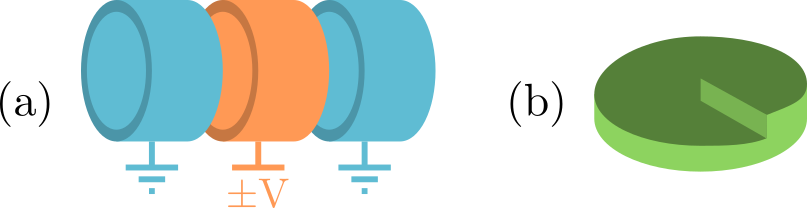
\includegraphics{einzel_and_ideal.png}
    \captionof{figure}{(a) Einzel čočka. (b) Ideální fázová destička.}
    \label{fig:einzel}
\end{Figure}

\section{Implementace}

Pro implementaci numerického výpočtu byl zvolen pythonovský notebook v prostředí Google Colab. Využili jsme knihovny \verb|numpy|, \verb|scipy| a \verb|plotly|.

Výpočty jsme prováděli pro několik fázových destiček s komplexní funkcí propustnosti (viz obr. \ref{fig:einzel_ideal} a \ref{fig:einzel_vysledek}). Nejprve bylo nutné funkci propustnosti nadefinovat. Konstanty byly voleny arbitrárně. Při modelování einzel čoček jsme každé čočce (kruhové i čtvercové) přiřadili fázi, která by ideálně odpovídala jejímu středu. 

Fourierovu transformaci jsme implementovali for cyklem, ve kterém jsme pro každý bod stínítka vypočetli Fraunhofferův difrakční integrál.
%\begin{equation}
%    \psi(x,y) = \left\langle  \exp\left( \dfrac{-\iu \,q_z}{f}y\,y'\right) \right| T(x',y') \left| \eul^{\left(\dfrac{-\iu \, q_z}{f}x\,x'\right)}\right\rangle
%\end{equation}

Pro tvorbu a úpravu obrázků byl využit program Inkscape.

\section{Výsledky}
    
První výpočet byl proveden pro ideální fázovou destičku (viz obr. \ref{fig:einzel_ideal}a,b). Při zvýšení topologického náboje můžeme pozorovat, jak se postupně zvětšuje poloměr hlavní maxima (v absolutní hodnotě) vlnové funkce. To odpovídá posunu prvního maxima modifikované Besselovy funkce se zvyšujícím se $l$. Toto chování pozorujeme i u dalších modelovaných fázových destiček.

V uspořádání einzel čoček do \uv{čtvercového čipu}  by se mohlo zdát, že abychom maximalizovali \uv{výtěžnost}, bude nejlepší využít celou plochu čtverce (obr. \ref{fig:einzel_ideal}c). Ve skutečnosti nám však čtvercová symetrie výsledek kazí. Výsledný svazek sice zjevně vorticitu vykazuje a přenáší tedy OAM, vlnová funkce však není radiálně symetrická a výpočty i měření by to značně komplikovalo. Podíváme-li se však na obr. \ref{fig:einzel_ideal}d,e, můžeme říci, že jednoduché zastínění rohových pixelů tak, aby byl \uv{čip} přibližně kruhový výsledek výrazně zlepšuje a takový vortex by již byl lépe použitelný. 

Úlohu jsme řešili také pro einzel čočky kruhového tvaru uspořádané na kružnici. Výsledky můžeme vidět na obr. \ref{fig:einzel_vysledek}. Vidíme, že pro $N = 4$ čočky se ještě výrazně projevuje čtyřčetná symetrie. Pro $N = 6$ je již ale výsledek uspokojivý. Pro vyšší $N$ se v tomto uspořádání sice vzdalujeme od transmisní funkce pro ideální destičku, neboť středem destičky nic neprochází, výsledky se však významně zlepšují s tím, jak jsou přechody mezi jednotlivými čočkami hladší. Toto můžeme výrazně pozorovat (inverzně) při přechodu od $l=1$ na $l=4$ pro $N=16$. Pro analytický popis svazku vzniklého difrakcí na einzel čočkách uspořádaných podél kružnice by již nestačila jednoduchá modifikovaná Besselova funkce a výsledek bychom museli vyjádřit komplikovanější řadou.

Nakonec poznamenejme, že vedlejší maxima všech výsledných vlnových funkcí ve skutečnosti nejsou tolik podstatná jako maximum hlavní. Vzhledem k tomu, že pozorovatelnou veličinou není sama vlnová funkce $\psi$, ale až hustota pravděpodobnosti $|\psi|^2$, pravděpodobnost nalezení elektronu mimo hlavní maximum je poměrně malá, neboť kvadrátem se vedlejší maxima významně utlumí.





\section*{Závěr}

Byl vytvořen numerický model přípravy elektronových vortexů pro několik typů fázových destiček. Zkoumali jsme ideální fázové destičky a destičky, které by bylo možné vytvořit s použitím tzv. einzel čoček. Pro ně byla transmisní funkce fázové destičky vytvořena ve třech modifikacích -- čtvercová síť s čtvercovými čočkami, kruhová síť s čtvercovými čočkami a kruhové čočky uspořádané podél kružnice. Kvalitativně jsme také zhodnotili použitelnost elektronových vortexů vzniknuvších na různých modelovaných fázových destičkách.




\end{multicols}

\begin{figure}
    \centering
    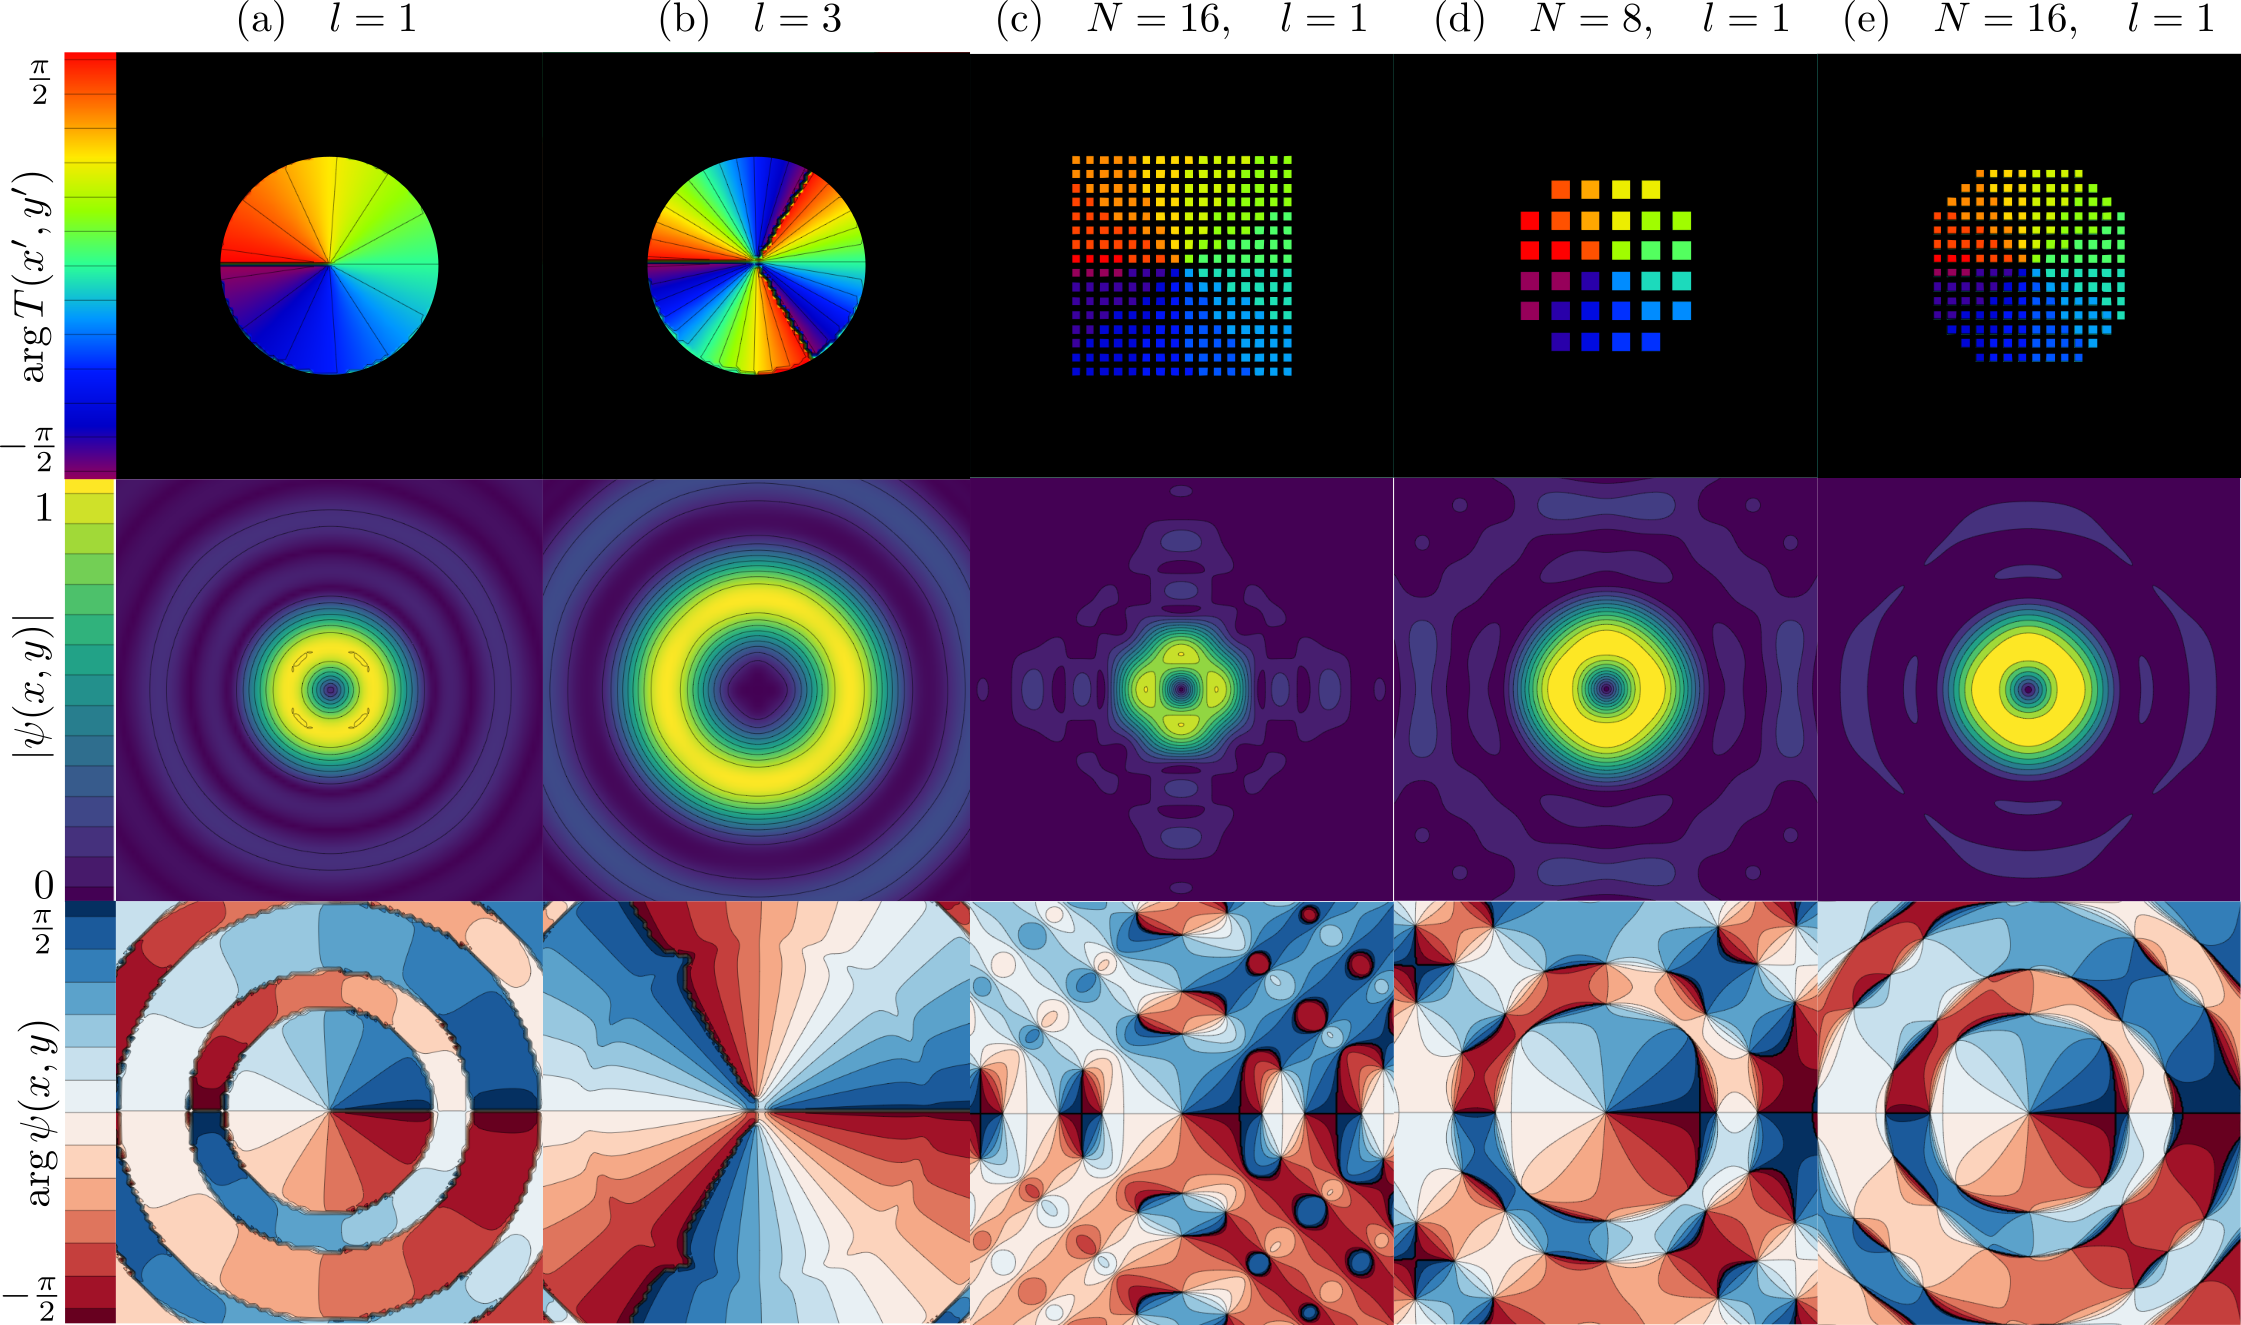
\includegraphics[width = \linewidth]{idealka_pixely_vysledek.png}
    \caption{Výsledky pro tvarování svazku pomocí (a, b) ideální fázové destičky; pomocí čtvercových einzel čoček -- pixelů uspořádaných ve čtvercové síti (c) v celém čtverci, (d, e) v kruhu. První řada: transmisní funkce fázové destičky. Druhá řada: absolutní hodnota vlnové funkce na stínítku normovaná k maximu. Třetí řada: fáze vlnové funkce na stínítku.}
    \label{fig:einzel_ideal}
\end{figure}

\begin{figure}
    \centering
    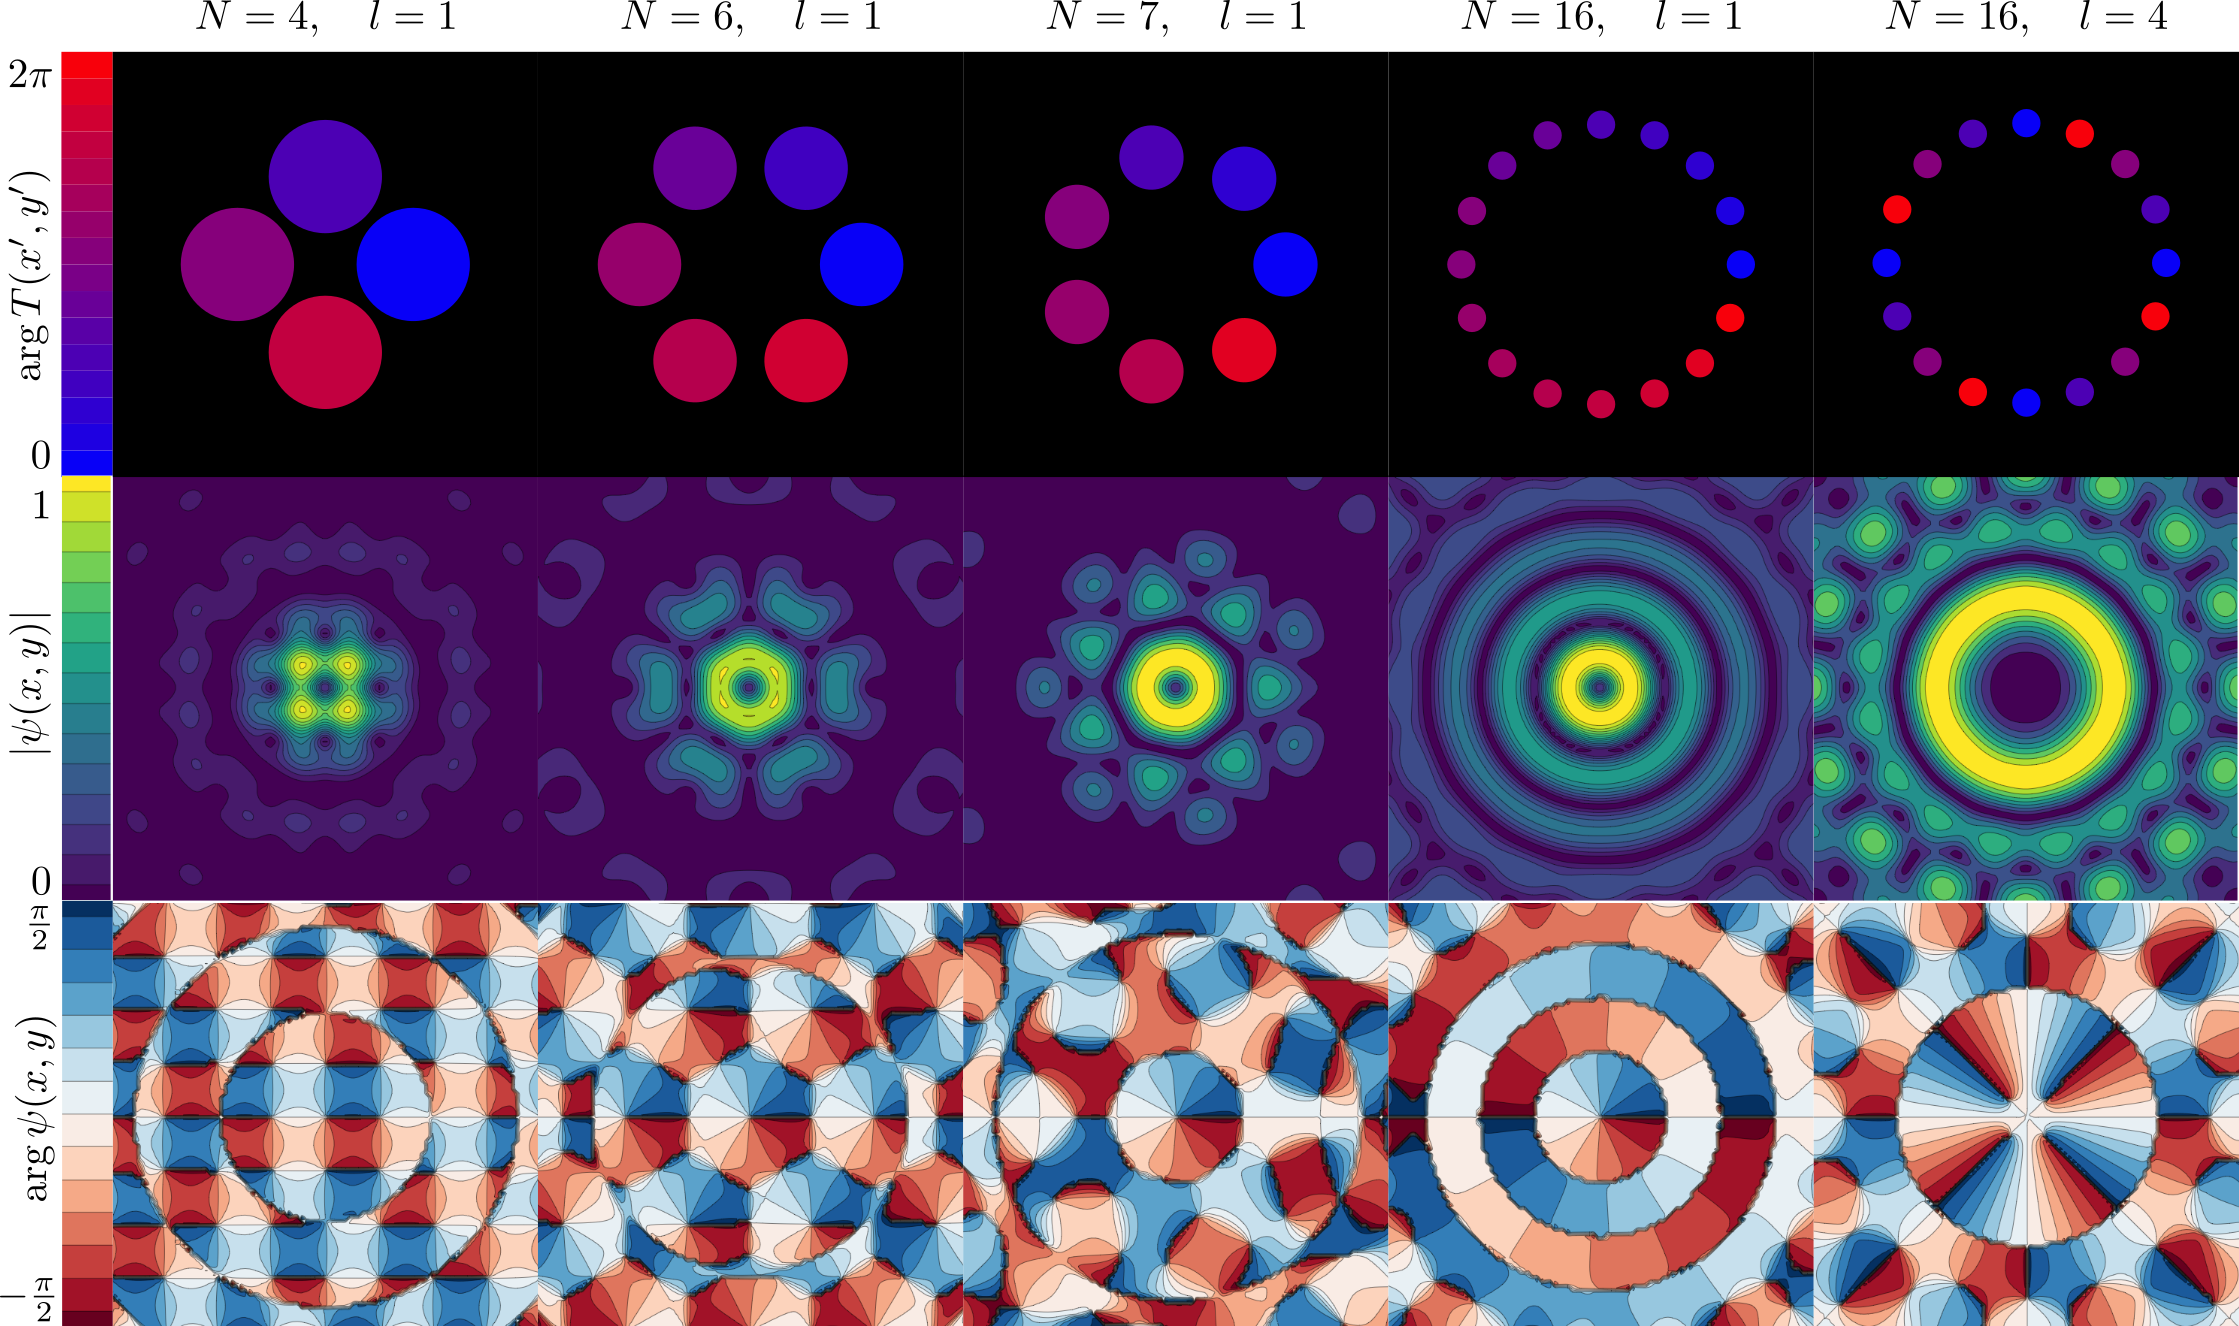
\includegraphics[width = \linewidth]{einzel_vysledek.png}
    \caption{Výsledky pro tvarování svazku pomocí einzel čoček uspořádaných podél kružnice. První řada: schematické uspořádání čoček s barvou odpovídající fázi, kterou získá vlnová funkce těsně za čočkou.  Druhá řada: absolutní hodnota vlnové funkce na stínítku normovaná k maximu. Třetí řada: fáze vlnové funkce na stínítku.}
    \label{fig:einzel_vysledek}
\end{figure}


\end{document}